\vspace*{-2mm}
\begin{table}[h]
    \scalebox{0.65}{
    \begin{subtable}[h]{0.35\textwidth}
        \centering
        \begin{tabular}{l|r|r|r}
        \backslashbox{\textbf{From}}{\textbf{To}} & \textbf{EU T4} & \textbf{US T4} & \textbf{US A10} \\ \hline
        \textbf{RTX8000}  & \cellcolor[HTML]{fadc24}0.45 & \cellcolor[HTML]{fa7e24}0.06 & \cellcolor[HTML]{fa7e24}0.05 \\ \hline
        \textbf{DGX-2 (8xV100)} & \cellcolor[HTML]{fadc24}0.55 & \cellcolor[HTML]{fa7e24}0.08 & \cellcolor[HTML]{fa7e24}0.07 
        \end{tabular}
        \caption{Single stream TCP throughput in Gbits.}
        \label{tab:local-experiments-bandwidth}
    \end{subtable}
    } 
    \scalebox{0.65}{ 
    \begin{subtable}[h]{0.35\textwidth}
        \centering   
        \begin{tabular}{l|r|r|r}
        \backslashbox{\textbf{From}}{\textbf{To}} & \textbf{EU T4} & \textbf{US T4} & \textbf{US A10} \\ \hline
        \textbf{RTX8000}  & \cellcolor[HTML]{fadc24}16.73 & \cellcolor[HTML]{fa7e24}150.80 & \cellcolor[HTML]{fa7e24}159.05 \\ \hline
        \textbf{DGX-2 (8xV100)} & \cellcolor[HTML]{fadc24}16.19 & \cellcolor[HTML]{fa7e24}150.27 & \cellcolor[HTML]{fa7e24}158.54
        \end{tabular}
        \caption{ICMP Latency in ms.}
        \label{tab:local-experiments-ping}
    \end{subtable}
    } 
    \caption{Average hybrid-cloud throughput and latency.}
    \label{tab:local-experiments-network}
    \vspace*{-8mm}
\end{table} 
\begin{table}[]
\vspace*{-4mm}
\begin{tabular}{r|r|r}
\textbf{Exp. Name}   & \textbf{Base Resource} & \textbf{Extra Resource} \\ \hline
\textbf{E-A-1,2,4,8} & RTX8000 EU      & T4 EU-\{1, 2, 4, 8\} \\
\textbf{E-B-1,2,4,8} &                 & T4 US-\{1, 2, 4, 8\} \\
\textbf{E-C-1,2,4,8} &                 & A10 US-\{1, 2, 4, 8\} \\ \hline
\textbf{F-A-1,2,4,8} & DGX-2 (8xV100) EU & T4 EU-\{1, 2, 4, 8\} \\
\textbf{F-B-1,2,4,8} &                 & T4 US-\{1, 2, 4, 8\} \\
\textbf{F-C-1,2,4,8} &                 & A10 US-\{1, 2, 4, 8\} \\
\end{tabular}
\caption{Setup for hybrid-cloud experiments.}
\label{tab:hybrid-cloud-experiments}
\vspace*{-8mm}
\end{table}
Can augmenting on-premise hardware with cloud resources be worthwhile to speed up DL training?
In this section, we examine two settings: \textbf{(E)}, where a consumer-grade GPU, the RTX8000, is deployed on-site, and \textbf{(F)}, where a server-grade node, the DGX-2 (8xV100), is deployed on-site (\Cref{tab:hybrid-cloud-experiments}).

\textbf{Experimental design.} In both settings, we want to investigate how to extend local hardware with cloud resources and when this leads to better throughput.
The cloud resources, in this case, are the same US/EU Google Cloud T4 instances as in ~\Cref{sec:geodistributed-performance} and the US LambdaLabs A10 GPUs from ~\Cref{sec:model-suitability}.
We double the number of cloud VMs with each increment, starting with one additional GPU (i.e., E-A-1) until we have eight additional cloud VMs (i.e., E-A-8). 
This allows us to compare the same hardware in the EU and the US, and slightly weaker, local hardware (EU T4) and better, but more distant hardware (US A10).

Both the \textbf{(E)} and \textbf{(F)} setups share the network uplink between 450 and 550 Mbits to the EU datacenter in Belgium, as they are located in the same building in Europe (\Cref{tab:local-experiments-network}). 
However, as this is not a Google-owned datacenter, the traffic is partly going over the public internet, which results in a lower bandwidth of 50 and 80 Mbits to the US-based VMs compared to 210 Mbits between the US and EU GC datacenters (\Cref{tab:geodistributed-throughput}).

\begin{figure}
    \begin{subfigure}[c]{0.24\textwidth}
        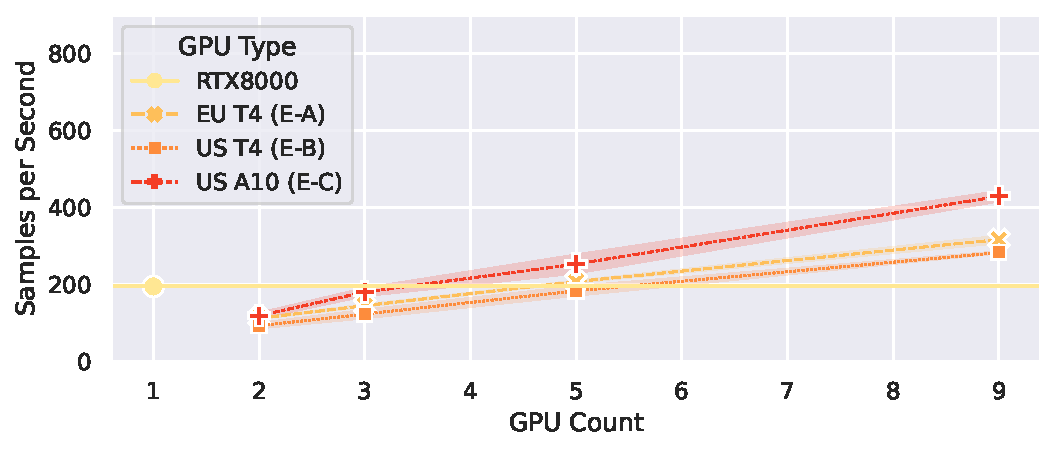
\includegraphics[width=\textwidth]{figures/misc/cv-private-setting-performance}
        \vspace{-15pt}
        \caption{CV Throughput}
        \label{fig:cv-private-hybrid-cloud-throughput}
    \end{subfigure}
    \begin{subfigure}[c]{0.21\textwidth}
        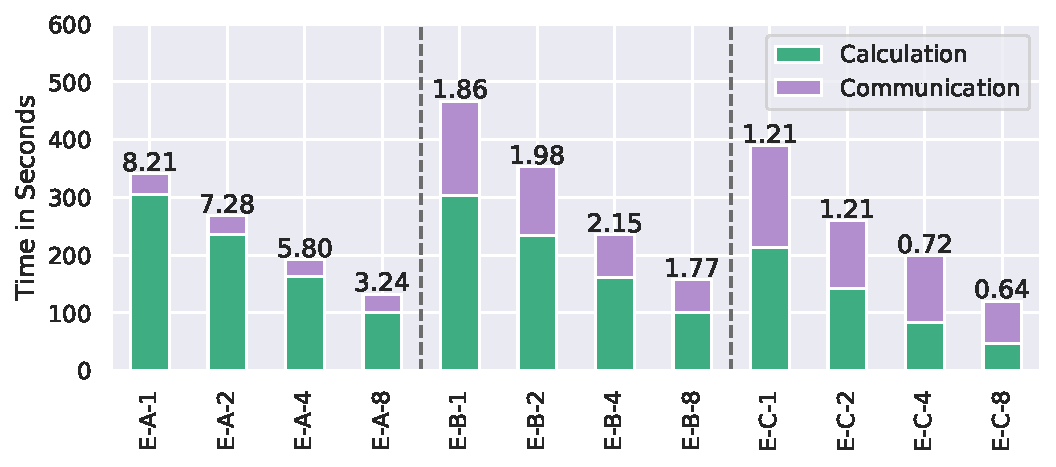
\includegraphics[width=\textwidth]{figures/misc/cv-private-cloud-performance-granularity}  
        \caption{CV Granularity}
        \label{fig:cv-private-hybrid-cloud-granularity}
    \end{subfigure}
        \begin{subfigure}[c]{0.24\textwidth}
        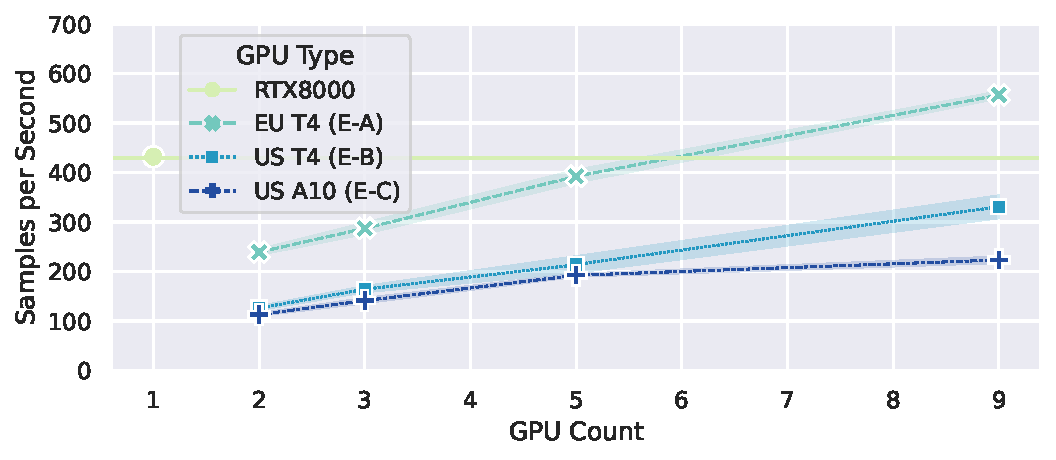
\includegraphics[width=\textwidth]{figures/misc/nlp-private-setting-performance}
        \vspace{-15pt}
        \caption{NLP Throughput}
        \label{fig:nlp-private-hybrid-cloud-throughput}
    \end{subfigure}
    \begin{subfigure}[c]{0.21\textwidth}
        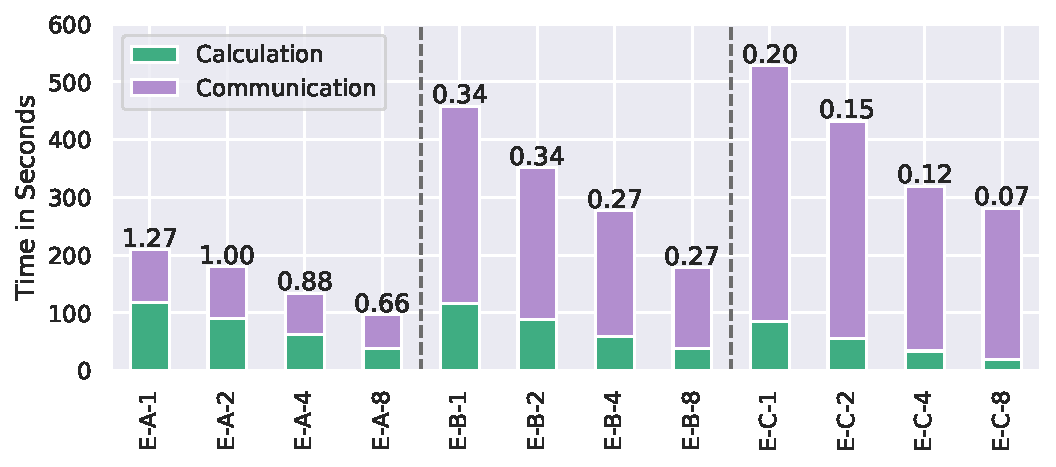
\includegraphics[width=\textwidth]{figures/misc/nlp-private-cloud-performance-granularity}  
        \caption{NLP Granularity} 
        \label{fig:nlp-private-hybrid-cloud-granularity}
    \end{subfigure}
    \vspace{-10pt}
    \caption{Hybrid-cloud experiments for the \textbf{(E)} setting.}
    \label{fig:private-hybrid-cloud-performance}
    \vspace*{-4mm}
\end{figure} 

\begin{table}[]
\begin{center}
\scalebox{0.8}{
\begin{tabular}{r|r|r|r|r|r|r}
 \backslashbox{\textbf{Model}}{\textbf{Setup}} & \textbf{RTX8000} & \textbf{E-A-8} & \textbf{E-B-8} & \textbf{E-C-8} & \textbf{8xT4} & \textbf{8xA10} \\ \hline
ConvNextLarge &   \cellcolor[HTML]{f17d3a}194.8 & \cellcolor[HTML]{f1be3a}316.8 & \cellcolor[HTML]{f1be3a}283.5 & \cellcolor[HTML]{c3f13a}429.3 & \cellcolor[HTML]{f1be3a}261.9 & \cellcolor[HTML]{67F13A}620.6 \\ \hline
RoBERTaXLM    &   \cellcolor[HTML]{f1be3a}431.8 & \cellcolor[HTML]{c3f13a}556.7 & \cellcolor[HTML]{f1be3a} 330.6 & \cellcolor[HTML]{f17d3a}223.7 & \cellcolor[HTML]{c3f13a}575.1 & \cellcolor[HTML]{67F13A}1059.9     
\end{tabular}
}
\end{center}
\caption{Hybrid-cloud vs. cloud-only throughput for the \textbf{(E)} setting.}
\label{tab:hybrid-vs-cloud-only-startup}
\vspace*{-5mm}
\end{table}

\textbf{(E) Consumer-grade setting.} The results follow the same trend as in ~\Cref{sec:geodistributed-performance}.
The CV task has a higher granularity of 8.21 with 2 GPUs at E-A-1 than NLP (1.27) (\Cref{fig:cv-private-hybrid-cloud-granularity,fig:nlp-private-hybrid-cloud-granularity}), and scales regardless of the location of the cloud resources (\Cref{fig:cv-private-hybrid-cloud-throughput}).
We almost match the baseline throughput of 195 SPS at 5 GPUs in all settings for CV (E-A-4, E-B-4, E-C-4).
The best throughput was reached at E-C-8 with the US A10 GPUs with 429 SPS.
For NLP, only the E-A-8 experiment beats the baseline with a speedup of 1.29x and 556 SPS due to the low granularity and the intercontinental base penalty for the US experiments.

However, is combining on-premise and remote cloud resources better than using the cloud without paying the intercontinental bandwidth tax?
To analyze this, we compare the \textbf{(E)} experiments with the 8xA10 experiment from ~\Cref{sec:model-suitability} and 8xT4 experiment from ~\Cref{sec:geodistributed-performance} in ~\Cref{tab:hybrid-vs-cloud-only-startup}.
First, the 8xA10 experiments are the fastest for both CV and NLP, which removes the respective hybrid-cloud combination from contention (E-C-8).
Second, the 8xT4 experiments for NLP are faster than any other hybrid-cloud setup, making the cloud-only solution favorable.
Finally, while we always beat the baseline 8xT4 CV throughput (261.9 SPS), but in the case of E-B-8 (283.5 SPS), just barely.
The throughput of E-A-8 (316.8 SPS) makes the hybrid-cloud setup the most favorable in terms of relative GPU scaling (32.5 SPS per GPU), but it does not come close to the best cloud-only throughput of 8xA10 with 620.6 SPS.

Summarizing, the cloud-only experiments are the fastest overall due to their single-GPU throughput and their locality.
Adding cloud resources to on-premise hardware leads to a high communication time, which is not compensated by the additional processing speed of the GPUs in our experiments.
Proximity to the on-premise hardware is essential, as the more local cloud resources (E-A-8) consistently resulted in a better throughput than the same remote cloud resources (E-B-8).

\begin{figure}
    \begin{subfigure}[c]{0.24\textwidth}
        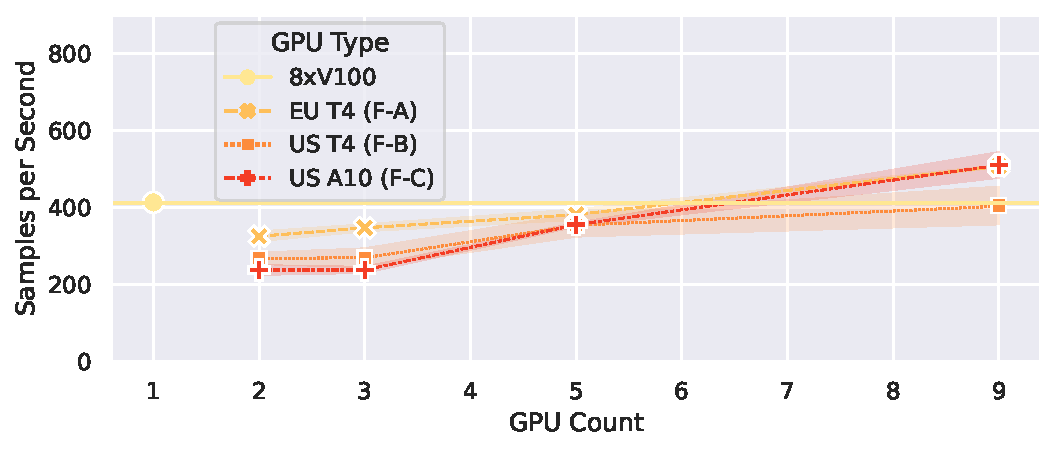
\includegraphics[width=\textwidth]{figures/misc/cv-research-setting-performance}
        \vspace{-15pt}
        \caption{CV Throughput} 
        \label{fig:cv-research-hybrid-cloud-throughput}
    \end{subfigure}
    \begin{subfigure}[c]{0.21\textwidth}
        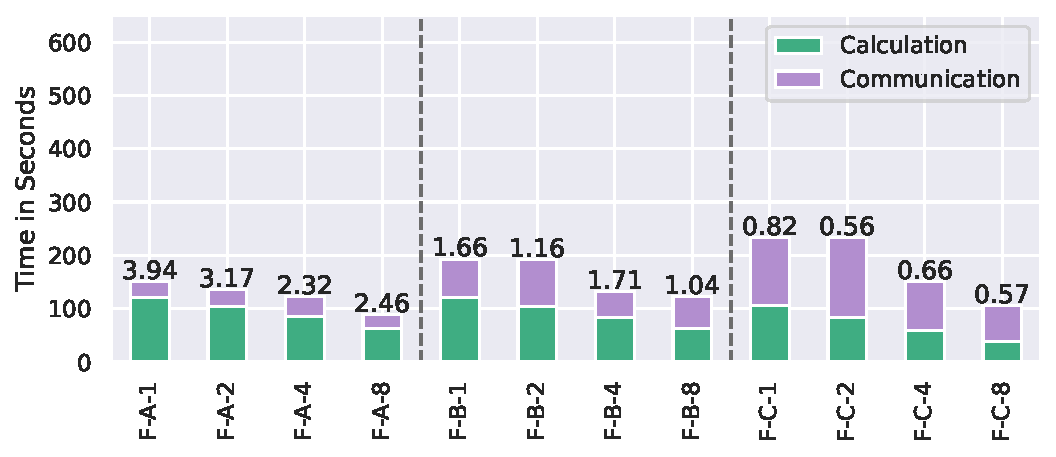
\includegraphics[width=\textwidth]{figures/misc/cv-research-cloud-performance-granularity}  
        %\vspace{-15pt}
        \caption{CV Granularity}
        \label{fig:cv-research-hybrid-cloud-granularity}
    \end{subfigure}
        \begin{subfigure}[c]{0.24\textwidth}
        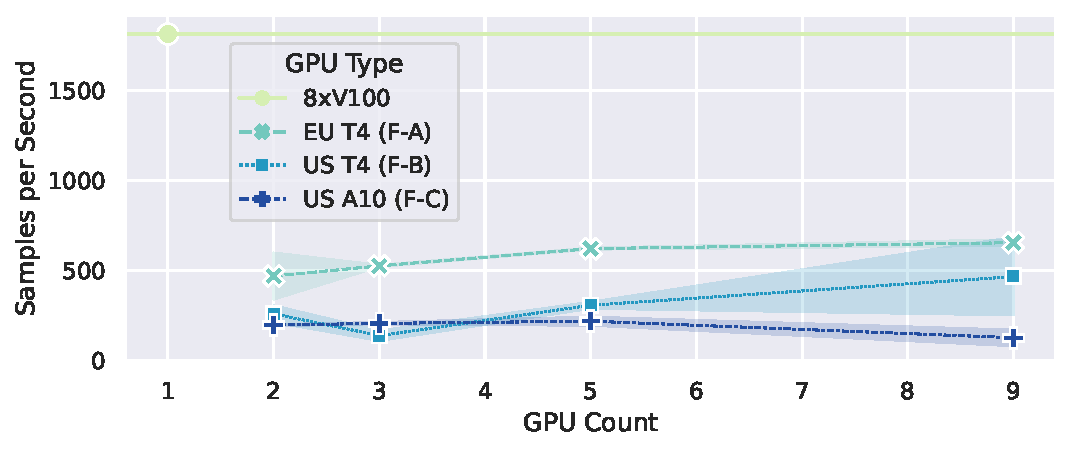
\includegraphics[width=\textwidth]{figures/misc/nlp-research-setting-performance}
        \vspace{-15pt} 
        \caption{NLP Throughput}
        \label{fig:nlp-research-hybrid-cloud-throughput}
    \end{subfigure}
    \begin{subfigure}[c]{0.21\textwidth}
        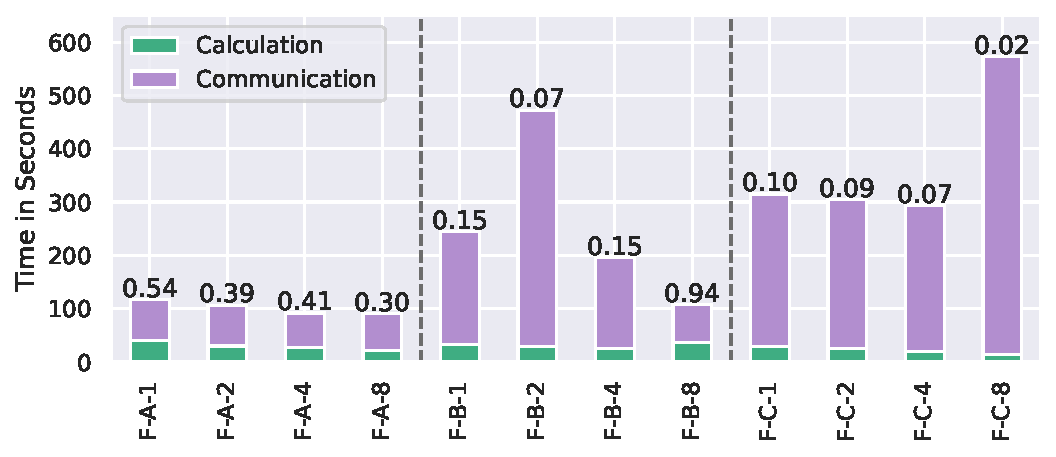
\includegraphics[width=\textwidth]{figures/misc/nlp-research-cloud-performance-granularity}  
        %\vspace{-15pt} 
        \caption{NLP Granularity} 
        \label{fig:nlp-research-hybrid-cloud-granularity}
    \end{subfigure}
    \vspace{-10pt}
    \caption{Hybrid-cloud experiments for the \textbf{(F)} setting.}
    \label{fig:research-hybrid-cloud-performance}
    \vspace*{-5mm}
\end{figure} 

\textbf{(F) Server-grade setting.} The baseline throughput is significantly higher compared to the RTX8000, with a much more powerful 8xV100 DGX node to 413~SPS for CV and 1811~SPS for NLP (\Cref{fig:cv-research-hybrid-cloud-throughput,fig:nlp-research-hybrid-cloud-throughput}).
This increases the penalties from ~\Cref{sec:model-suitability}, leading to the only speedup from baseline for CV in experiments F-A-8 (507~SPS) and F-C-8 (510~SPS).
This is surprising, as the older T4 GPUs in the EU perform similarly to the much newer A10 GPUs in the US, showcasing the trade-off between slower, local compute and faster, remote compute.
The granularity of 2.46 for F-A-8 shows that there is enough calculation time to distribute, while the F-C-8 experiments spend $\approx 62\%$ of the total training time on communication with a granularity of 0.57 (\Cref{fig:cv-research-hybrid-cloud-granularity}).
The NLP experiments never reach the baseline throughput of the 8xV100 due to using most of the time for communication. 
The NLP F-B and F-C experiments mainly consist of communication (\Cref{fig:nlp-research-hybrid-cloud-granularity}) with a granularity of up to 0.02, which results in a nonlinear, unstable training time due to the minimum matchmaking time issue \textbf{(2)} from ~\Cref{sec:model-suitability}.

In summary, the hybrid-cloud experiments conclude that while on-premise hardware can be augmented with cloud resources, it will likely be cost-efficient if all resources are on the same continent.
Using only cloud resources is more advantageous if the on-premises hardware is not co-located.